\section{GenericArbiter Class Reference}
\label{classGenericArbiter}\index{GenericArbiter@{GenericArbiter}}
{\tt \#include $<$genericArbiter.h$>$}

Collaboration diagram for GenericArbiter:\nopagebreak
\begin{figure}[H]
\begin{center}
\leavevmode
\includegraphics[height=400pt]{classGenericArbiter__coll__graph}
\end{center}
\end{figure}
\subsection*{Public Member Functions}
\begin{CompactItemize}
\item 
{\bf GenericArbiter} ()
\item 
{\bf $\sim$GenericArbiter} ()
\item 
bool {\bf is\_\-requested} ({\bf uint} ch)
\item 
bool {\bf is\_\-empty} ()
\item 
void {\bf set\_\-no\_\-requestors} ({\bf uint} ch)
\item 
void {\bf request} ({\bf uint} ch)
\item 
{\bf uint} {\bf get\_\-no\_\-requestors} ()
\item 
{\bf uint} {\bf pick\_\-winner} ()
\item 
string {\bf toString} () const 
\item 
void {\bf clear\_\-winner} ()
\end{CompactItemize}
\subsection*{Public Attributes}
\begin{CompactItemize}
\item 
{\bf uint} {\bf node\_\-ip}
\item 
{\bf uint} {\bf address}
\item 
string {\bf name}
\end{CompactItemize}
\subsection*{Private Attributes}
\begin{CompactItemize}
\item 
{\bf uint} {\bf vcs}
\item 
vector$<$ bool $>$ {\bf requests}
\item 
{\bf uint} {\bf last\_\-winner}
\item 
bool {\bf done}
\end{CompactItemize}


\subsection{Detailed Description}


Definition at line 30 of file genericArbiter.h.

\subsection{Constructor \& Destructor Documentation}
\index{GenericArbiter@{GenericArbiter}!GenericArbiter@{GenericArbiter}}
\index{GenericArbiter@{GenericArbiter}!GenericArbiter@{GenericArbiter}}
\subsubsection[{GenericArbiter}]{\setlength{\rightskip}{0pt plus 5cm}GenericArbiter::GenericArbiter ()}\label{classGenericArbiter_f268b17257b6084b8faa82e4539580f5}




Definition at line 23 of file genericArbiter.cc.

References address, done, last\_\-winner, name, and node\_\-ip.\index{GenericArbiter@{GenericArbiter}!$\sim$GenericArbiter@{$\sim$GenericArbiter}}
\index{$\sim$GenericArbiter@{$\sim$GenericArbiter}!GenericArbiter@{GenericArbiter}}
\subsubsection[{$\sim$GenericArbiter}]{\setlength{\rightskip}{0pt plus 5cm}GenericArbiter::$\sim$GenericArbiter ()}\label{classGenericArbiter_c8e72db9c3fb2c9b406933a104592519}




Definition at line 32 of file genericArbiter.cc.

\subsection{Member Function Documentation}
\index{GenericArbiter@{GenericArbiter}!clear\_\-winner@{clear\_\-winner}}
\index{clear\_\-winner@{clear\_\-winner}!GenericArbiter@{GenericArbiter}}
\subsubsection[{clear\_\-winner}]{\setlength{\rightskip}{0pt plus 5cm}void GenericArbiter::clear\_\-winner ()}\label{classGenericArbiter_137758be6498b8dc717cf4d4c8bc56be}




Definition at line 84 of file genericArbiter.cc.

References done, last\_\-winner, and requests.

Referenced by GenericInterfaceVcs::handle\_\-tick\_\-event().

Here is the caller graph for this function:\nopagebreak
\begin{figure}[H]
\begin{center}
\leavevmode
\includegraphics[width=420pt]{classGenericArbiter_137758be6498b8dc717cf4d4c8bc56be_icgraph}
\end{center}
\end{figure}
\index{GenericArbiter@{GenericArbiter}!get\_\-no\_\-requestors@{get\_\-no\_\-requestors}}
\index{get\_\-no\_\-requestors@{get\_\-no\_\-requestors}!GenericArbiter@{GenericArbiter}}
\subsubsection[{get\_\-no\_\-requestors}]{\setlength{\rightskip}{0pt plus 5cm}{\bf uint} GenericArbiter::get\_\-no\_\-requestors ()}\label{classGenericArbiter_8c0d21bfde4ea6968d2a5d404215dd65}




Definition at line 73 of file genericArbiter.cc.

References requests, and vcs.\index{GenericArbiter@{GenericArbiter}!is\_\-empty@{is\_\-empty}}
\index{is\_\-empty@{is\_\-empty}!GenericArbiter@{GenericArbiter}}
\subsubsection[{is\_\-empty}]{\setlength{\rightskip}{0pt plus 5cm}bool GenericArbiter::is\_\-empty ()}\label{classGenericArbiter_334fbdb8fc6071936b0d05a5778cc714}




Definition at line 62 of file genericArbiter.cc.

References requests, and vcs.

Referenced by GenericInterfaceVcs::handle\_\-tick\_\-event().

Here is the caller graph for this function:\nopagebreak
\begin{figure}[H]
\begin{center}
\leavevmode
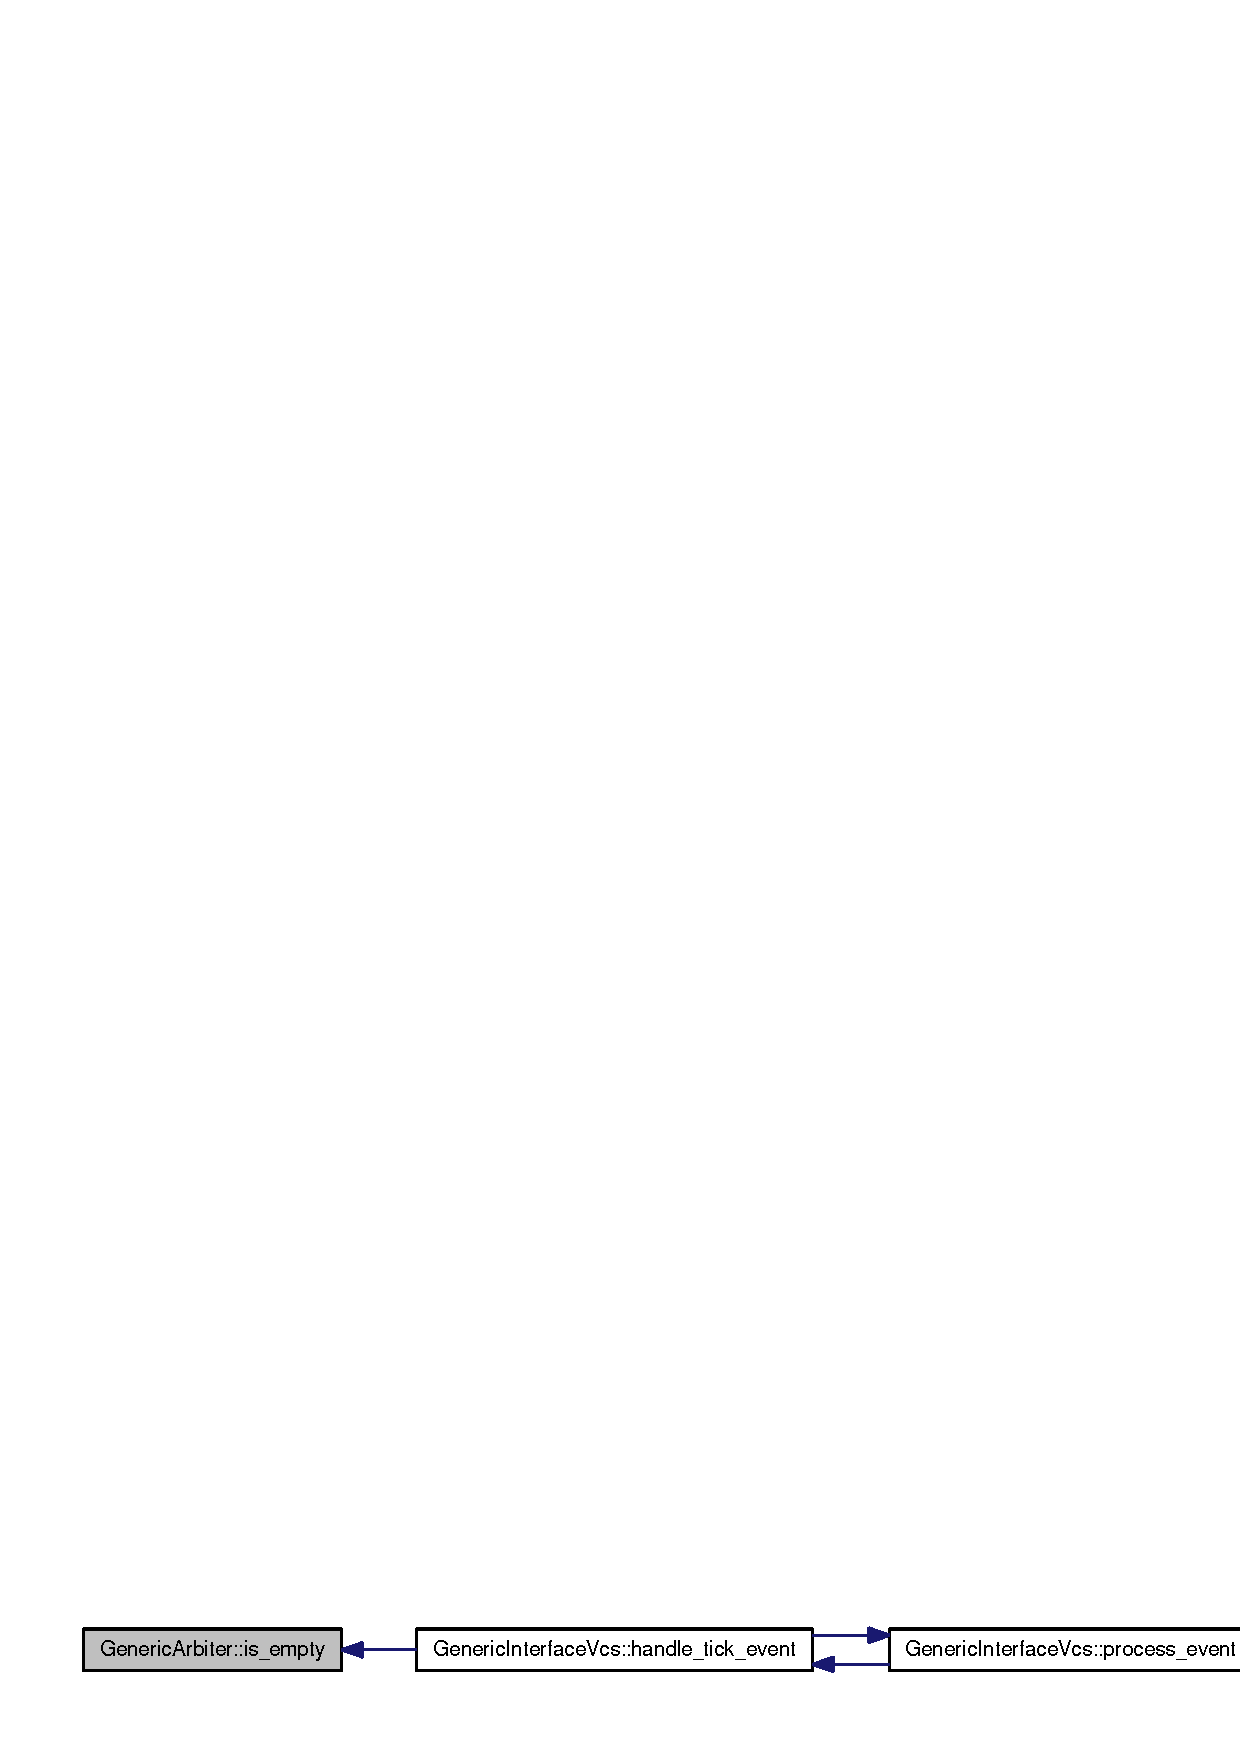
\includegraphics[width=417pt]{classGenericArbiter_334fbdb8fc6071936b0d05a5778cc714_icgraph}
\end{center}
\end{figure}
\index{GenericArbiter@{GenericArbiter}!is\_\-requested@{is\_\-requested}}
\index{is\_\-requested@{is\_\-requested}!GenericArbiter@{GenericArbiter}}
\subsubsection[{is\_\-requested}]{\setlength{\rightskip}{0pt plus 5cm}bool GenericArbiter::is\_\-requested ({\bf uint} {\em ch})}\label{classGenericArbiter_6cb1ab1819bd58fc51935af5af5bd6d5}




Definition at line 55 of file genericArbiter.cc.

References requests.

Referenced by GenericInterfaceVcs::handle\_\-tick\_\-event().

Here is the caller graph for this function:\nopagebreak
\begin{figure}[H]
\begin{center}
\leavevmode
\includegraphics[width=420pt]{classGenericArbiter_6cb1ab1819bd58fc51935af5af5bd6d5_icgraph}
\end{center}
\end{figure}
\index{GenericArbiter@{GenericArbiter}!pick\_\-winner@{pick\_\-winner}}
\index{pick\_\-winner@{pick\_\-winner}!GenericArbiter@{GenericArbiter}}
\subsubsection[{pick\_\-winner}]{\setlength{\rightskip}{0pt plus 5cm}{\bf uint} GenericArbiter::pick\_\-winner ()}\label{classGenericArbiter_4a5b38f3d16471a75c0c35fc1ecb3031}




Definition at line 92 of file genericArbiter.cc.

References done, last\_\-winner, and requests.

Referenced by GenericInterfaceVcs::handle\_\-tick\_\-event().

Here is the caller graph for this function:\nopagebreak
\begin{figure}[H]
\begin{center}
\leavevmode
\includegraphics[width=420pt]{classGenericArbiter_4a5b38f3d16471a75c0c35fc1ecb3031_icgraph}
\end{center}
\end{figure}
\index{GenericArbiter@{GenericArbiter}!request@{request}}
\index{request@{request}!GenericArbiter@{GenericArbiter}}
\subsubsection[{request}]{\setlength{\rightskip}{0pt plus 5cm}void GenericArbiter::request ({\bf uint} {\em ch})}\label{classGenericArbiter_88ab811caecaf5738fc32143a35a482f}




Definition at line 47 of file genericArbiter.cc.

References done, and requests.

Referenced by GenericInterfaceVcs::handle\_\-tick\_\-event().

Here is the caller graph for this function:\nopagebreak
\begin{figure}[H]
\begin{center}
\leavevmode
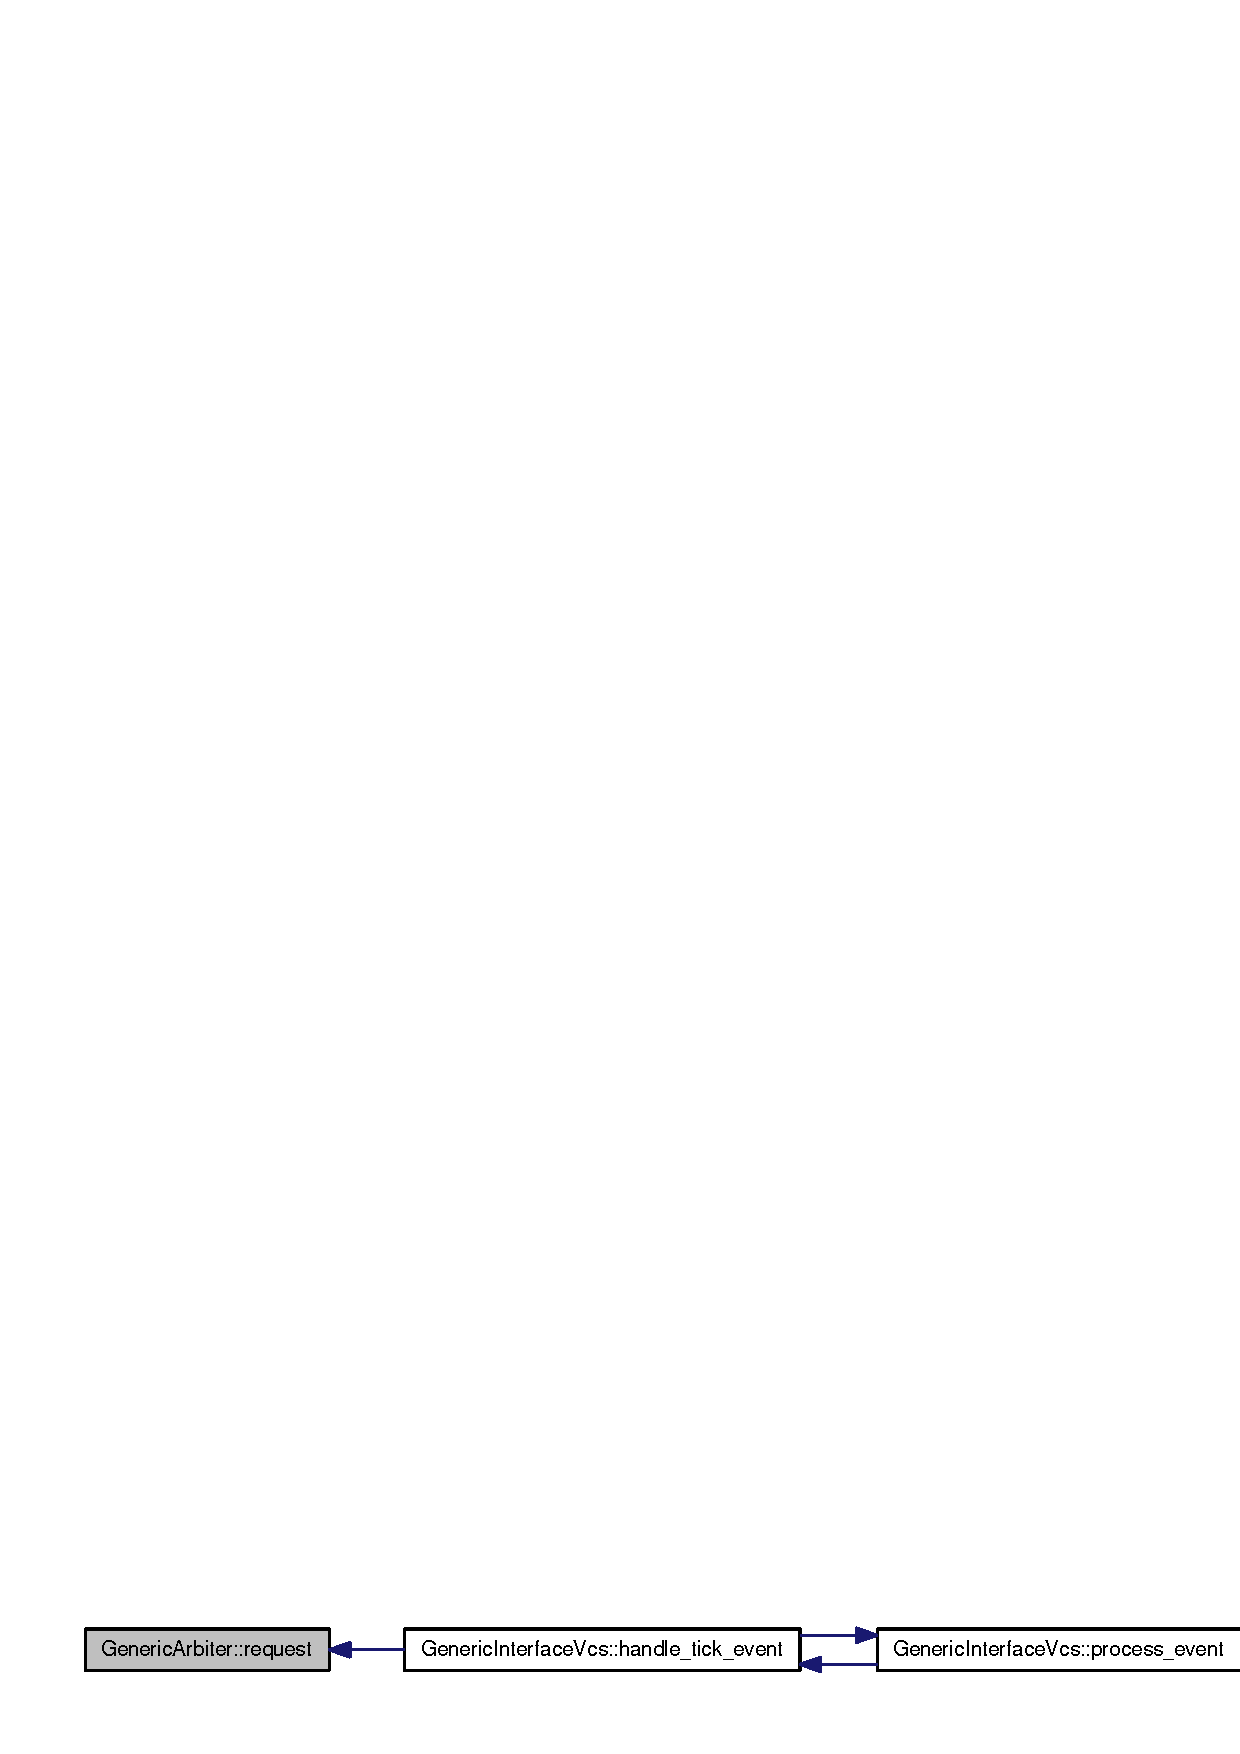
\includegraphics[width=414pt]{classGenericArbiter_88ab811caecaf5738fc32143a35a482f_icgraph}
\end{center}
\end{figure}
\index{GenericArbiter@{GenericArbiter}!set\_\-no\_\-requestors@{set\_\-no\_\-requestors}}
\index{set\_\-no\_\-requestors@{set\_\-no\_\-requestors}!GenericArbiter@{GenericArbiter}}
\subsubsection[{set\_\-no\_\-requestors}]{\setlength{\rightskip}{0pt plus 5cm}void GenericArbiter::set\_\-no\_\-requestors ({\bf uint} {\em ch})}\label{classGenericArbiter_3994d2b032f4774b73c923c78c05d81a}




Definition at line 38 of file genericArbiter.cc.

References requests, and vcs.

Referenced by GenericInterfaceVcs::setup().

Here is the caller graph for this function:\nopagebreak
\begin{figure}[H]
\begin{center}
\leavevmode
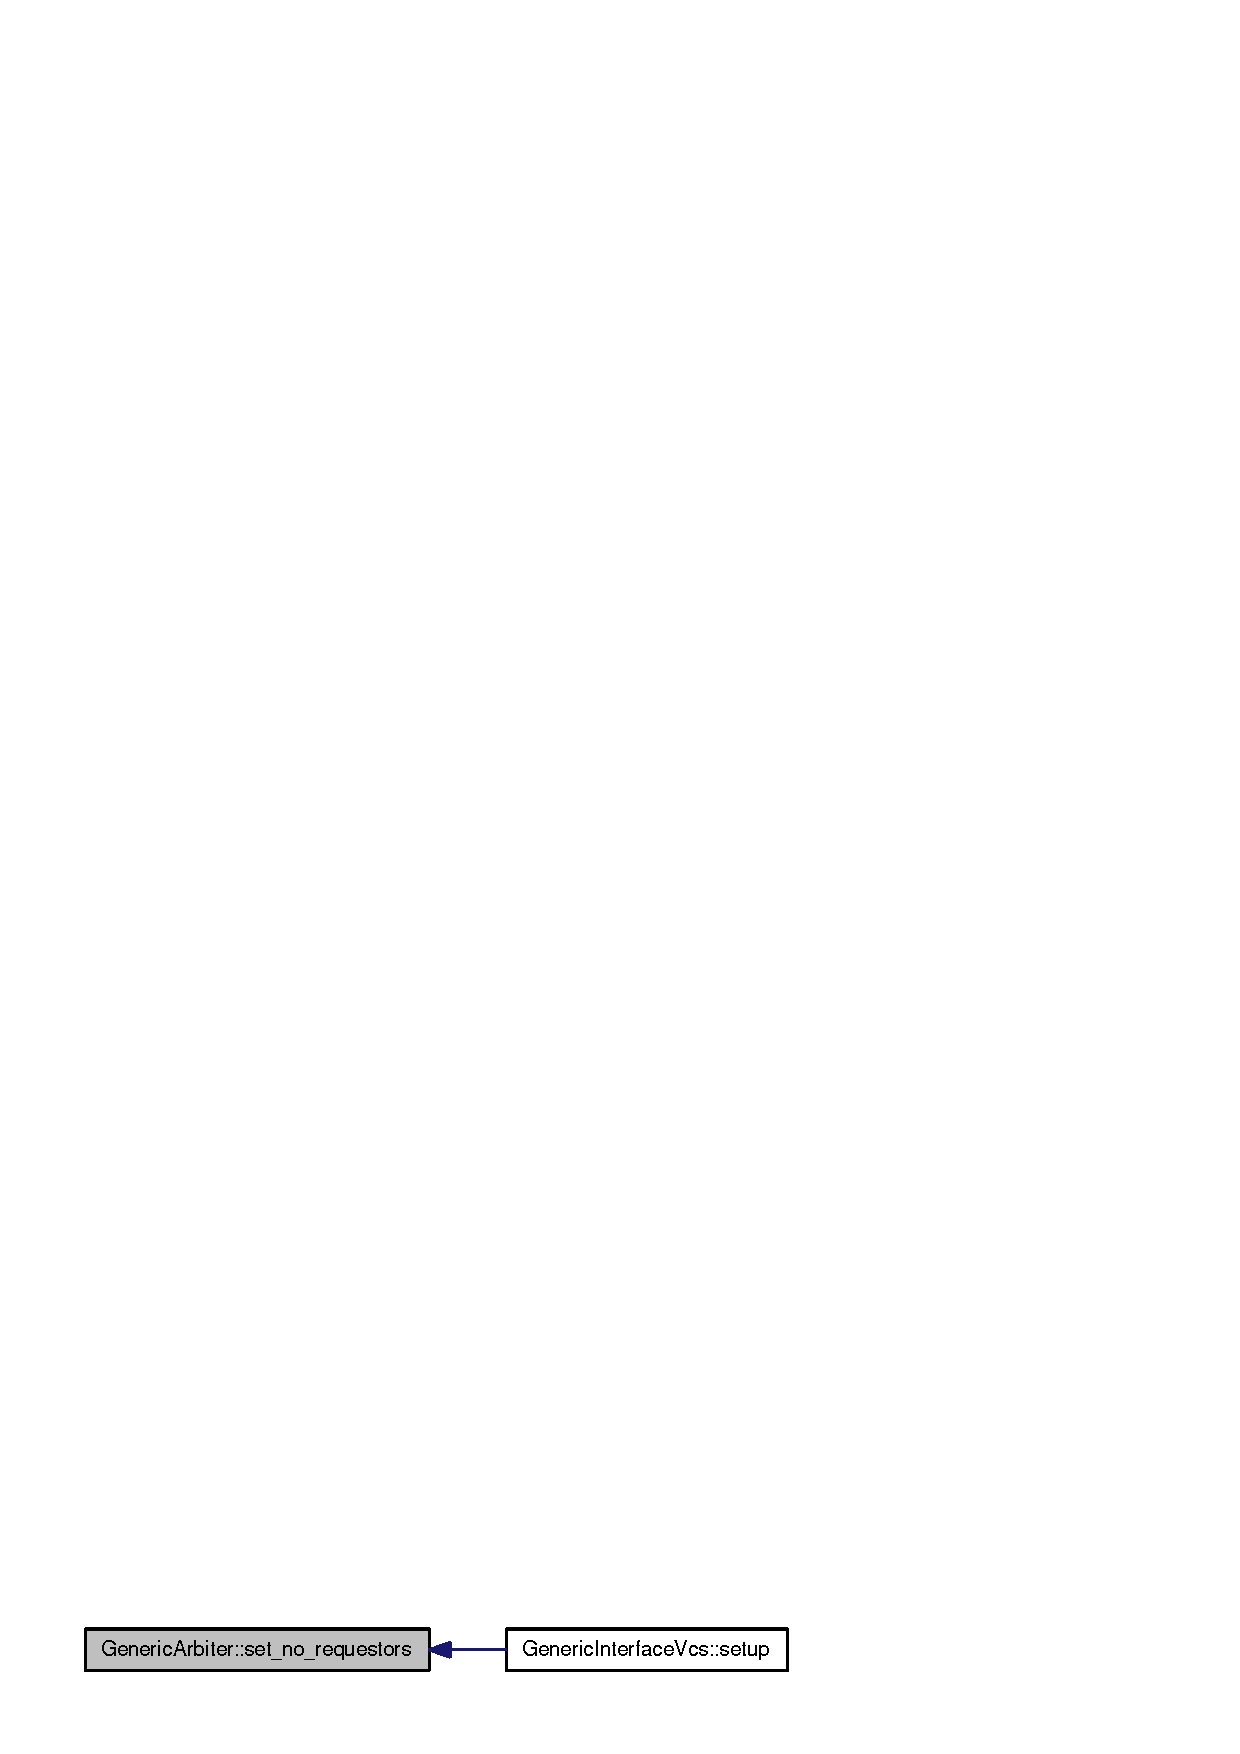
\includegraphics[width=191pt]{classGenericArbiter_3994d2b032f4774b73c923c78c05d81a_icgraph}
\end{center}
\end{figure}
\index{GenericArbiter@{GenericArbiter}!toString@{toString}}
\index{toString@{toString}!GenericArbiter@{GenericArbiter}}
\subsubsection[{toString}]{\setlength{\rightskip}{0pt plus 5cm}string GenericArbiter::toString () const}\label{classGenericArbiter_dfd7645d22ce13eb428e73fd9fa34b63}




Definition at line 120 of file genericArbiter.cc.

References last\_\-winner, and requests.

\subsection{Member Data Documentation}
\index{GenericArbiter@{GenericArbiter}!address@{address}}
\index{address@{address}!GenericArbiter@{GenericArbiter}}
\subsubsection[{address}]{\setlength{\rightskip}{0pt plus 5cm}{\bf uint} {\bf GenericArbiter::address}}\label{classGenericArbiter_d570be8e0435c540c11f46cd9e68d8fc}




Definition at line 36 of file genericArbiter.h.

Referenced by GenericArbiter().\index{GenericArbiter@{GenericArbiter}!done@{done}}
\index{done@{done}!GenericArbiter@{GenericArbiter}}
\subsubsection[{done}]{\setlength{\rightskip}{0pt plus 5cm}bool {\bf GenericArbiter::done}\hspace{0.3cm}{\tt  [private]}}\label{classGenericArbiter_b7f37783b4ef2d2ba15ed6e12b493e91}




Definition at line 53 of file genericArbiter.h.

Referenced by clear\_\-winner(), GenericArbiter(), pick\_\-winner(), and request().\index{GenericArbiter@{GenericArbiter}!last\_\-winner@{last\_\-winner}}
\index{last\_\-winner@{last\_\-winner}!GenericArbiter@{GenericArbiter}}
\subsubsection[{last\_\-winner}]{\setlength{\rightskip}{0pt plus 5cm}{\bf uint} {\bf GenericArbiter::last\_\-winner}\hspace{0.3cm}{\tt  [private]}}\label{classGenericArbiter_531eb0c84fe9433d923f0d73da3aab24}




Definition at line 52 of file genericArbiter.h.

Referenced by clear\_\-winner(), GenericArbiter(), pick\_\-winner(), and toString().\index{GenericArbiter@{GenericArbiter}!name@{name}}
\index{name@{name}!GenericArbiter@{GenericArbiter}}
\subsubsection[{name}]{\setlength{\rightskip}{0pt plus 5cm}string {\bf GenericArbiter::name}}\label{classGenericArbiter_d58995bf70e8e6b7422ab4e7bd97e360}




Definition at line 37 of file genericArbiter.h.

Referenced by GenericArbiter().\index{GenericArbiter@{GenericArbiter}!node\_\-ip@{node\_\-ip}}
\index{node\_\-ip@{node\_\-ip}!GenericArbiter@{GenericArbiter}}
\subsubsection[{node\_\-ip}]{\setlength{\rightskip}{0pt plus 5cm}{\bf uint} {\bf GenericArbiter::node\_\-ip}}\label{classGenericArbiter_970eebd92edf4b43bd34dbe378aee0b4}




Definition at line 35 of file genericArbiter.h.

Referenced by GenericArbiter().\index{GenericArbiter@{GenericArbiter}!requests@{requests}}
\index{requests@{requests}!GenericArbiter@{GenericArbiter}}
\subsubsection[{requests}]{\setlength{\rightskip}{0pt plus 5cm}vector$<$ bool $>$ {\bf GenericArbiter::requests}\hspace{0.3cm}{\tt  [private]}}\label{classGenericArbiter_11d312f8174346c263f24a3795d3d813}




Definition at line 51 of file genericArbiter.h.

Referenced by clear\_\-winner(), get\_\-no\_\-requestors(), is\_\-empty(), is\_\-requested(), pick\_\-winner(), request(), set\_\-no\_\-requestors(), and toString().\index{GenericArbiter@{GenericArbiter}!vcs@{vcs}}
\index{vcs@{vcs}!GenericArbiter@{GenericArbiter}}
\subsubsection[{vcs}]{\setlength{\rightskip}{0pt plus 5cm}{\bf uint} {\bf GenericArbiter::vcs}\hspace{0.3cm}{\tt  [private]}}\label{classGenericArbiter_afc0b7f094d6ee2d8ba620e2bed141f4}




Definition at line 50 of file genericArbiter.h.

Referenced by get\_\-no\_\-requestors(), is\_\-empty(), and set\_\-no\_\-requestors().

The documentation for this class was generated from the following files:\begin{CompactItemize}
\item 
{\bf genericArbiter.h}\item 
{\bf genericArbiter.cc}\end{CompactItemize}
